\subsection{First error found}
The first error we encountered when simulating our processor design in ModelSim
\cite{modelsim}, was an error where \emph{pipeline\_stage1} gives an undefined
value as output every second clockcycle.
\paragraph*{}
Figure \ref{fig:error-1-text} below illustrates the problem:
\begin{figure}[h]
	\caption{First error (you can view it fullscale in the appendix:
\ref{fig:error-1-landscape}).}
	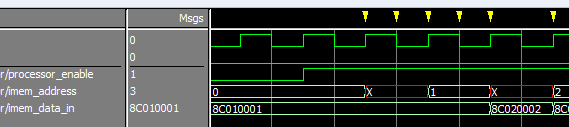
\includegraphics[scale=0.5]{figures/pc_error_annenhver_LITEN.png}
	\label{fig:error-1-text}
\end{figure}

\paragraph*{}
This problem was caused by the program counter's input in
\emph{pipeline\_stage1} not being properly connected to the adder incrementing
program counter's output. This problem was resolved by connecting the output
from the adder correctly into the multiplexor choosing between the adder and
branch values as inputs for the program counter.

\subsection{Second error found}
The second error encountered was when simulating the entire pipeline design as
a whole to check whether instructions as a whole propagated correctly.
\paragraph*{}
It was discovered (as figure \ref{fig:error-2-text} illustrates) that due to the
bottom signal ``stage\_4\_out\_wb'' being undeclared until the ALU operations unit
sends the load/store command to the ALU. The ``stage\_4\_out\_wb'' should not
have gotten the value 1 (logical high), before the signal ``alu\_mem\_mux\_out''
gets the value 2. Since it becomes logical high before this point, the
consequence is that garbage is written back to the registers in
\emph{pipeline\_stage2}.
\begin{figure}[H]
	\caption{Second error (you can view it fullscale in the appendix:
\ref{fig:error-2-landscape})}
	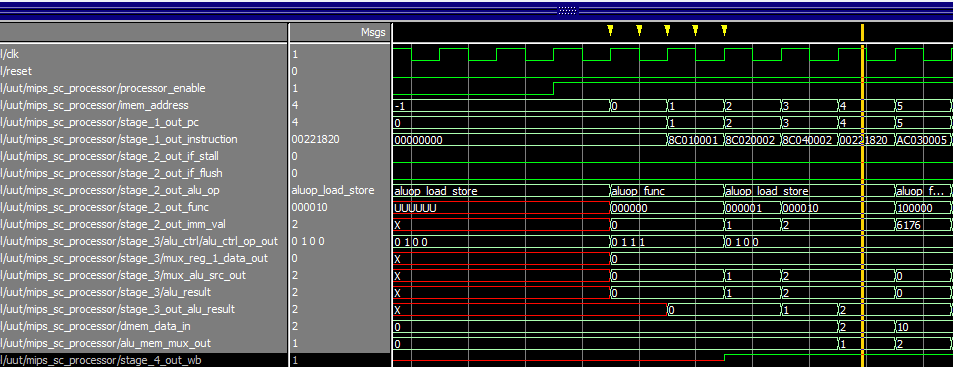
\includegraphics[scale=0.5]{figures/error_2.png}
	\label{fig:error-2-text}
\end{figure}

\paragraph*{}
This was never resolved. It was deemed to be a minor issue at first since it only occured during the first few cycles of the simulation. Then it was discovered that it was probably a symptom of a larger timing issue where the write back signal was set too early. There was also a correct value that only appeared for half a clock cycle before disappearing which was never written back to registers. This points to a larger timing issue which we were not able to resolve.

\subsection{First test}
\begin{figure}[H]
	\caption{First test. See also appendix section \ref{fig:test-1-landscape}).}
	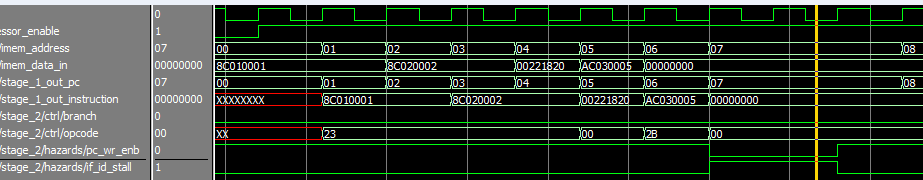
\includegraphics[scale=0.6]{figures/test_1_text.png}
	\label{fig:test-1-text}
\end{figure}

The first test we ran, as opposed to errors we encountered, was to test if the
stall functionality worked correctly with the program counter in \emph{
pipeline\_stage1}.
\paragraph*{}
Figure \ref{fig:test-1-text} illustrates how when the stall signal
``if\_id\_stall'' becomes one (logical high), the program counter's write-enable
signal ``pc\_wr\_enb'' turns off by becoming zero.
\paragraph*{}
The correct result of these actions are shown by the signals ``imem\_address''
and ``stage\_1\_out\_pc''. You can see that before the stall signal turns on,
these two aforementioned signal values increment on each clock cycle. Yet when
the stall signals turns on, they keep their value, and only continue
incrementing after it stall has been turned off again by reverting to zero.
